%%%%%%%%%%%%%%%%%%%%%%%%%%%%%%%%%%%%%%%%%
% Structured General Purpose Assignment
% LaTeX Template
%
% This template has been downloaded from:
% http://www.latextemplates.com
%
% Original author:
% Ted Pavlic (http://www.tedpavlic.com)
%
% Note:
% The \lipsum[#] commands throughout this template generate dummy text
% to fill the template out. These commands should all be removed when
% writing assignment content.
%
%%%%%%%%%%%%%%%%%%%%%%%%%%%%%%%%%%%%%%%%%

%----------------------------------------------------------------------------------
%   PACKAGES AND OTHER DOCUMENT CONFIGURATIONS
%----------------------------------------------------------------------------------

\documentclass{article}

\usepackage[utf8]{inputenc}
\usepackage[spanish]{babel}
\usepackage{fancyhdr} % Required for custom headers
\usepackage{lastpage} % Required to determine the last page for the footer
\usepackage{graphicx} % Required to insert images
\usepackage{tikz}
\usepackage[export]{adjustbox}
\usepackage{enumitem}
\usepackage{environ}
\usepackage{multicol}
\usepackage{hyperref}
\usepackage[font=small]{caption}
\usepackage{pifont}
\selectlanguage{spanish}
\addto\extrasspanish{%
    \def\figureautorefname{Figura}%
}
\newcommand{\myarrow}{\ding{223}}
\newcommand{\cmark}{\ding{51}}
\newcommand{\xmark}{\ding{55}}

% Margins
\topmargin=-0.45in
\evensidemargin=0in
\oddsidemargin=0in
\textwidth=6.5in
\textheight=9.0in
\headsep=0.25in

\linespread{1.1} % Line spacing

% Set up the header and footer
\pagestyle{fancy}
\lhead{\small \hmwkClass: \hmwkTitle} % Top left header
\chead{} % Top center header
\rhead{\small \hmwkAuthorName} % Top right header
\lfoot{} % Bottom left footer
\cfoot{} % Bottom center footer
\rfoot{Página\ \thepage\ de\ \pageref{LastPage}} % Bottom right footer
\renewcommand\headrulewidth{0.4pt} % Size of the header rule
\renewcommand\footrulewidth{0.4pt} % Size of the footer rule

\setlength\parindent{0pt} % Removes all indentation from paragraphs
\setlength{\multicolsep}{6.0pt plus 2.0pt minus 1.5pt} % 50% of original values

\newlength\widest
\makeatletter
\NewEnviron{ldescription}{%
    \vbox{%
        \global\setlength\widest{0pt}%
        \def\item[##1]{%
            \settowidth\@tempdima{\textbf{##1}}%
            \ifdim \@tempdima>\widest \global\setlength\widest{\@tempdima} \fi%
        }%
        \setbox0=\hbox{\BODY}%
    }
    \begin{description}[leftmargin=\dimexpr\widest+0.5em\relax,labelindent=0pt, labelwidth=\widest]
        \BODY
\end{description}%
}
\makeatother

%----------------------------------------------------------------------------------
%   NAME AND CLASS SECTION
%----------------------------------------------------------------------------------

\newcommand{\hmwkTitle}{Práctica\ 2} % Assignment title
\newcommand{\hmwkClass}{Sistemas Informáticos I} % Course/class
\newcommand{\hmwkClassTime}{10:30am} % Class/lecture time
\newcommand{\hmwkAuthorName}{\small Sergio Fuentes de Uña | Daniel Perdices Burrero} % Your name

%----------------------------------------------------------------------------------
%   TITLE PAGE
%----------------------------------------------------------------------------------

\title{
    \vspace{2in}
    \textmd{\textbf{\hmwkClass:\ \hmwkTitle}}\\
    \vspace{0.1in}
    \begin{center}
        \begin{tikzpicture}
            \begin{scope}
                \clip [rounded corners=12pt] (0,0) rectangle coordinate (centerpoint) (160pt,40pt);
                \node [inner sep=0pt] at (centerpoint) {
\includegraphics[width=160pt]{betabet}};
            \end{scope}
        \end{tikzpicture}
    \end{center}
    \vspace{3in}
}

\author{\textbf{\hmwkAuthorName}}

%----------------------------------------------------------------------------------

\begin{document}

\maketitle

%----------------------------------------------------------------------------------
%   TABLE OF CONTENTS
%----------------------------------------------------------------------------------

%\setcounter{tocdepth}{1} % Uncomment this line if you don't want subsections listed in the ToC

\newpage
\tableofcontents
\newpage

\section{Archivos}
La entrega final de la práctica está compuesta por los siguientes archivos:
\begin{ldescription}
    \item[$\bullet$ \texttt{index.php}]
        Página principal del sitio web.
    \item[$\bullet$ \texttt{matches.php}]
        Listado y búsqueda de encuentros disponibles para apostar.
    \item[$\bullet$ \texttt{register.php}]
        Formulario de registro de un nuevo usuario.
    \item[$\bullet$ \texttt{bet.php}]
        Formulario de realización y modificación de una apuesta.
    \item[$\bullet$ \texttt{checkout.php}]
        Administración del carrito de apuestas.
    \item[$\bullet$ \texttt{credit.php}]
        Administración de saldo del usuario.
    \item[$\bullet$ \texttt{history.php}]
        Historial de apuestas del usuario.
    \item[$\bullet$ \texttt{usercount.php}]
        Banner con el número de usuarios conectados.
    \item[$\bullet$ \texttt{theme.css}]
        Hoja de estilo CSS del sitio web.
    \item[$\bullet$ \texttt{functions.js}]
        Librería de funciones JavaScript.
    \item[$\bullet$ \texttt{db.xml}]
        Conjunto de apuestas disponibles en XML.
    \item[$\bullet$ \texttt{users/}]
        Directorio de datos de los usuarios.
    \item[$\bullet$ \texttt{games/}]
        Directorio de recursos gráficos para las apuestas.
    \item[$\bullet$ \texttt{images/}]
        Directorio de recursos gráficos de propósito general.
    \item[$\bullet$ \texttt{Memoria-P2.pdf}]
        Memoria del trabajo realizado (este archivo).
\end{ldescription}
\newpage
\section{Instrucciones de uso}
\subsection{Encontrar una apuesta}
Al acceder a la página principal se muestra el conjunto de todas las apuestas, organizadas en dos secciones:
\begin{itemize}
    \item\textbf{\textit{Upcoming Matches}}: Encuentros que aún no se han celebrado o que aún no han terminado y por los que se puede apostar, los más inminentes aparecen primero.
        \smallbreak
        \begin{minipage}{\linewidth}
            \centering
            \captionsetup{type=figure}
            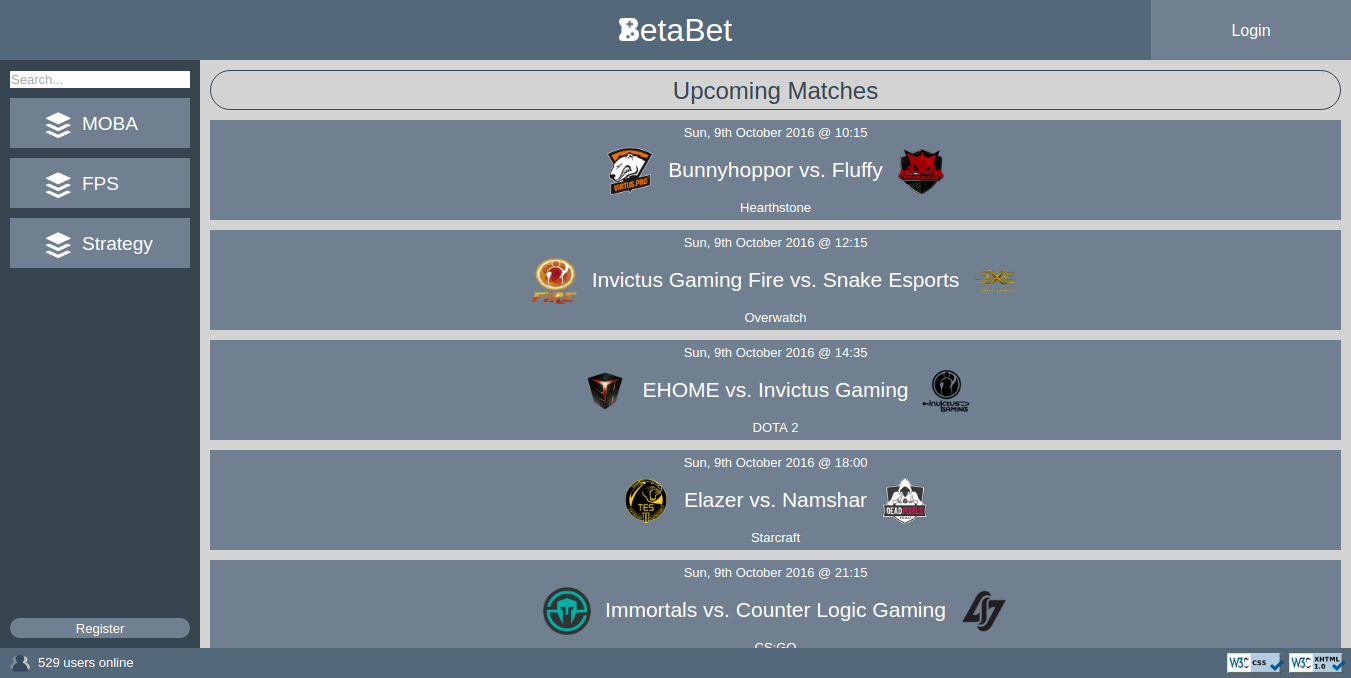
\includegraphics[width=\linewidth]{fig1}
            \caption{\textit{Upcoming Matches}}
            \label{fig:fig1}
        \end{minipage}
    \item\textbf{\textit{Latest Matches}}: Encuentros finalizados por los que ya no es posible apostar y cuyos resultados se indican en la página, los más recientes aparecen primero.\
        \smallbreak
        \begin{minipage}{\linewidth}
            \centering
            \captionsetup{type=figure}
            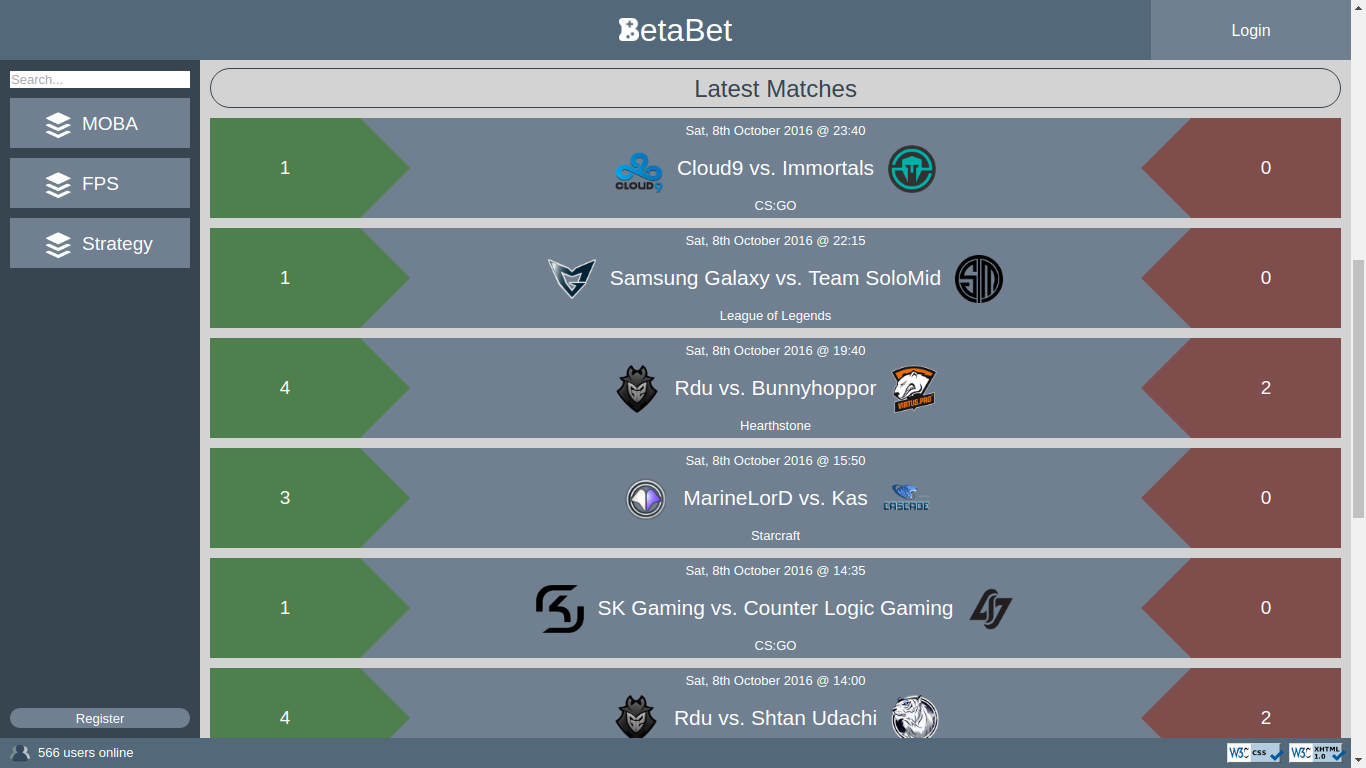
\includegraphics[width=\linewidth]{fig2}
            \caption{\textit{Latest Matches}}
            \label{fig:fig2}
        \end{minipage}
\end{itemize}
\newpage
Existen dos mecanismos de filtrado de apuestas para localizar encuentros según unos intereses determinados:
\begin{itemize}
    \item\textbf{Categorías}: Desplegando los menús del panel lateral y pulsando los botones correspondientes es posible mostrar únicamente las apuestas de una cierta categoría.
        \smallbreak
        \begin{minipage}{\linewidth}
            \centering
            \captionsetup{type=figure}
            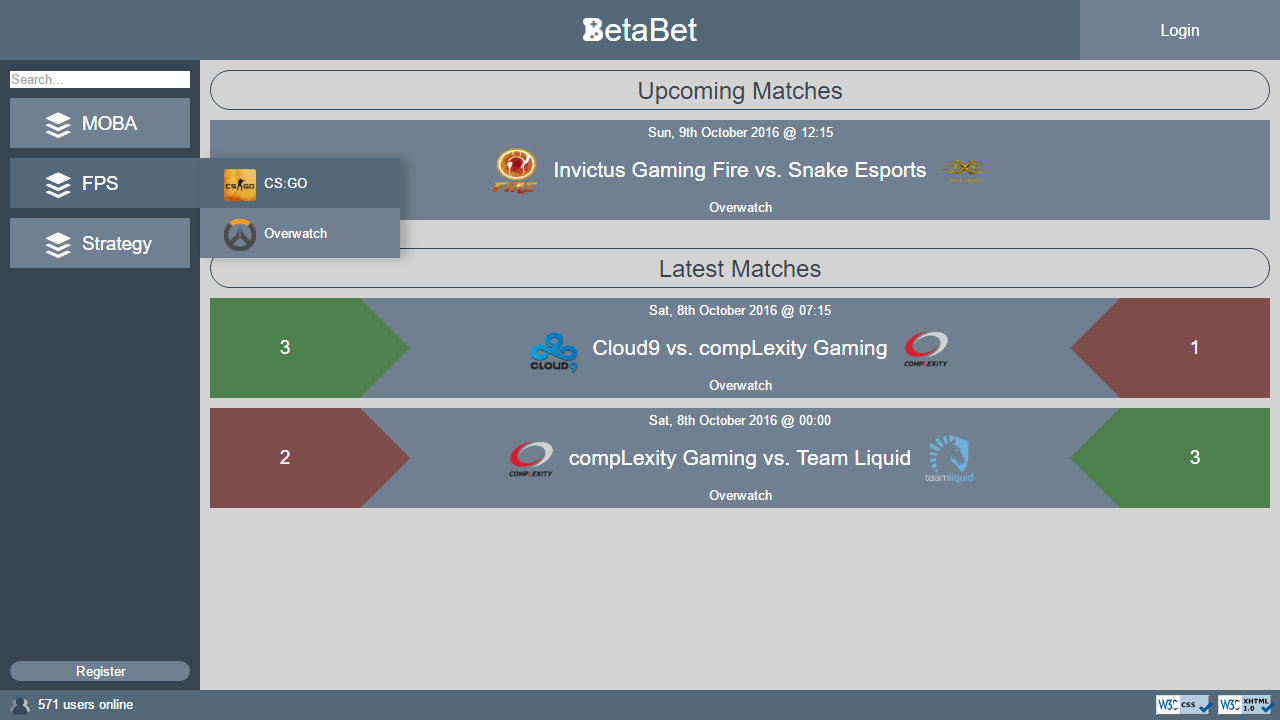
\includegraphics[width=\linewidth]{fig3}
            \caption{Filtrado por categorías}
            \label{fig:fig3}
        \end{minipage}
    \item\textbf{Búsqueda}: Escribiendo directamente en el campo de búsqueda del panel lateral se filtran automáticamente las apuestas cuyos datos coinciden con el patrón buscado.
        \smallbreak
        \begin{minipage}{\linewidth}
            \centering
            \captionsetup{type=figure}
            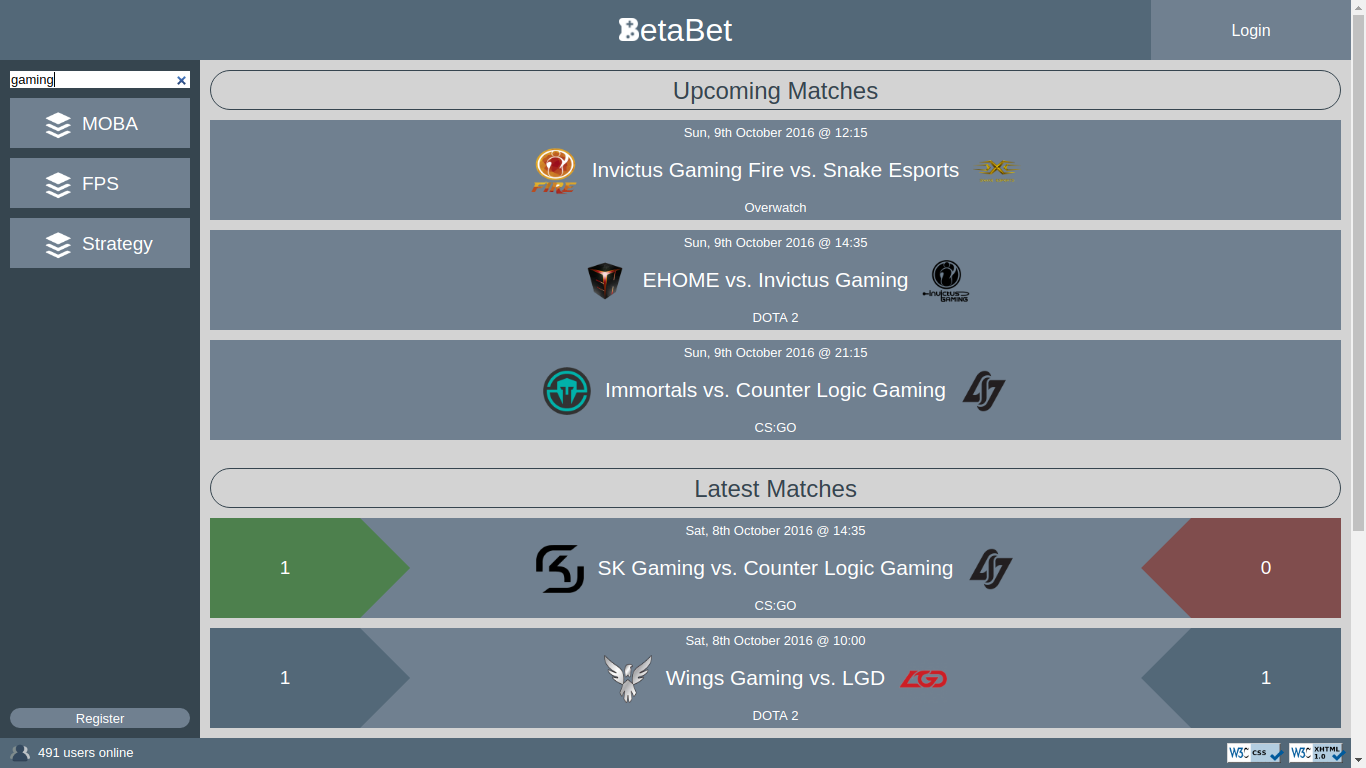
\includegraphics[width=\linewidth]{fig4}
            \caption{Filtrado por búsqueda}
            \label{fig:fig4}
        \end{minipage}
\end{itemize}
\newpage
\subsection{Realizar una apuesta}
Una vez localizada la apuesta deseada, basta con hacer clic en ella para acceder al formulario de apuesta.
\smallbreak
\begin{minipage}{\linewidth}
    \centering
    \captionsetup{type=figure}
    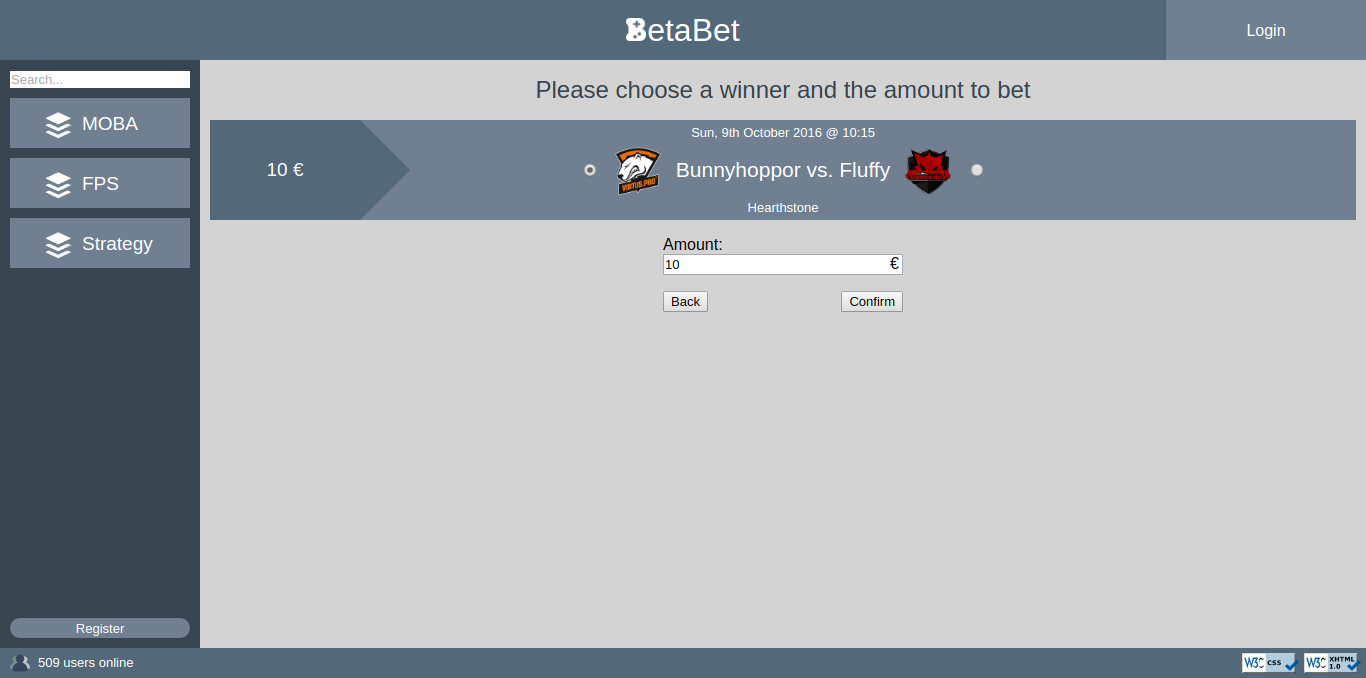
\includegraphics[width=\linewidth]{fig5}
    \caption{Formulario de apuesta}
    \label{fig:fig5}
\end{minipage}
\smallbreak
Tras confirmar un ganador y una cantidad para apostar, se comprueba la validez de los datos introducidos.
\begin{multicols}{4}
    \begin{center}
        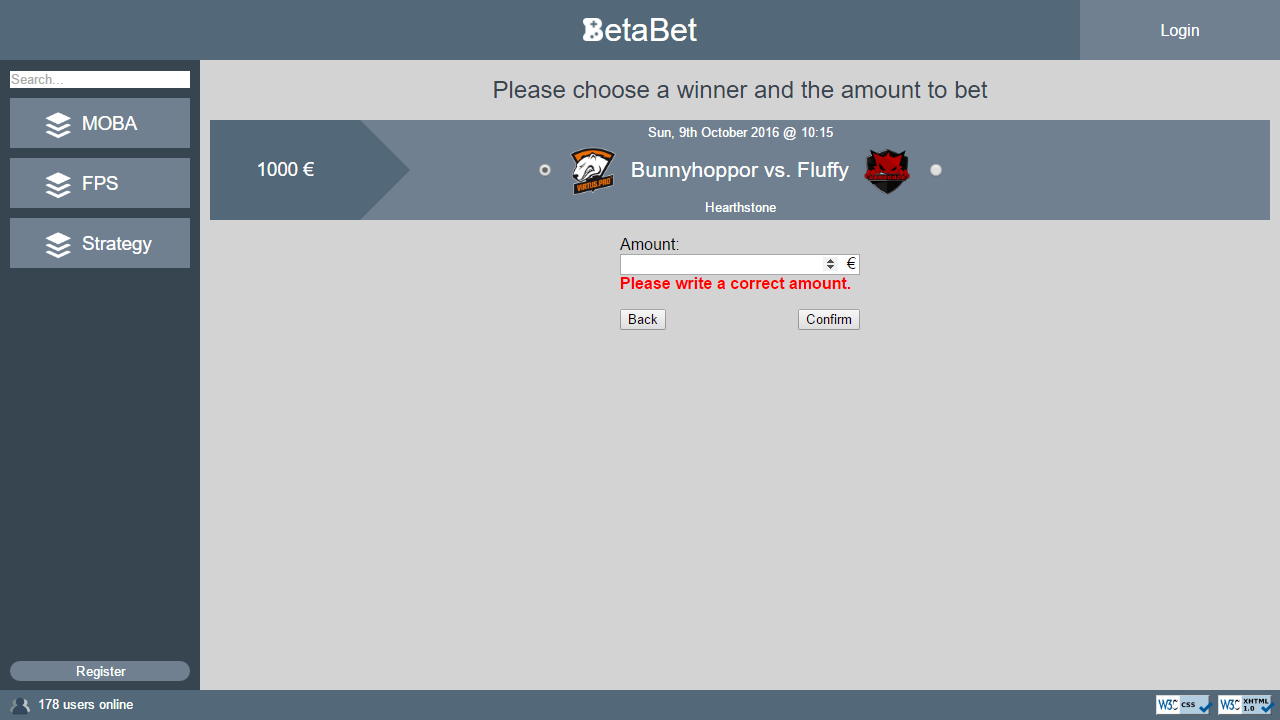
\includegraphics[width=.975\linewidth]{bet1}
        Formato incorrecto
    \end{center}
    \columnbreak
    \begin{center}
        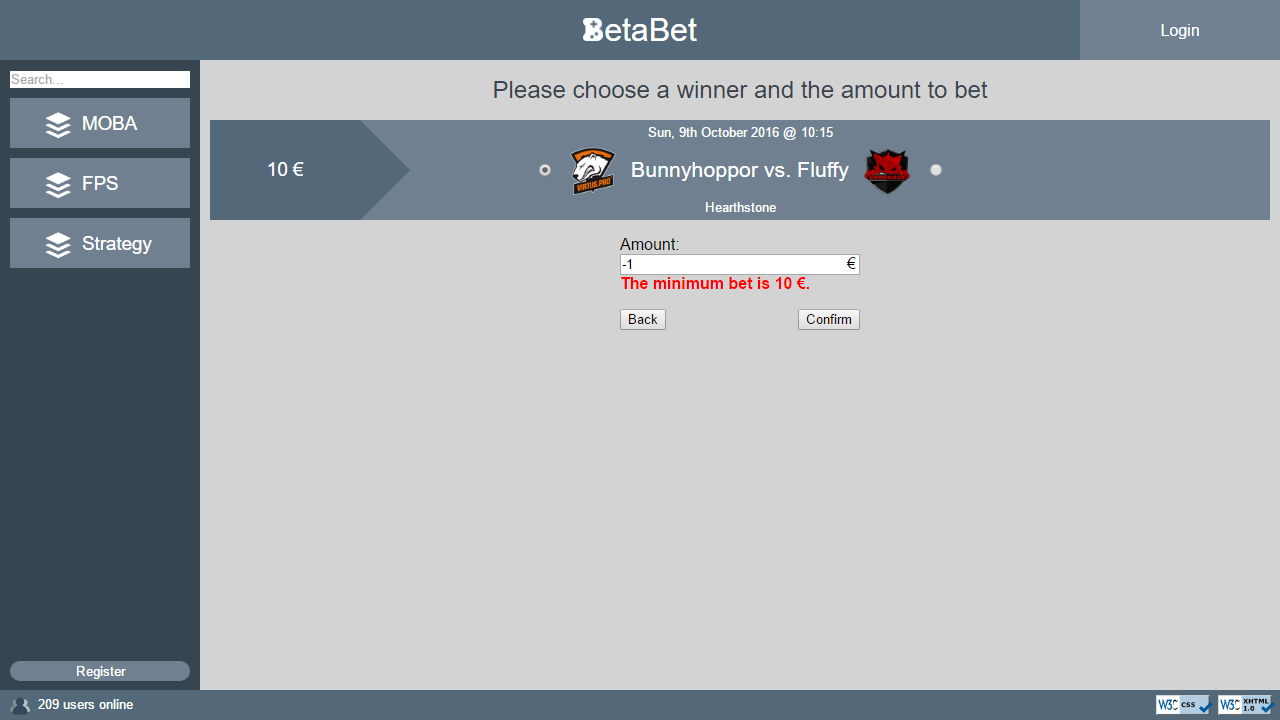
\includegraphics[width=.975\linewidth]{bet2}
        Apuesta muy pequeña
    \end{center}
    \columnbreak
    \begin{center}
        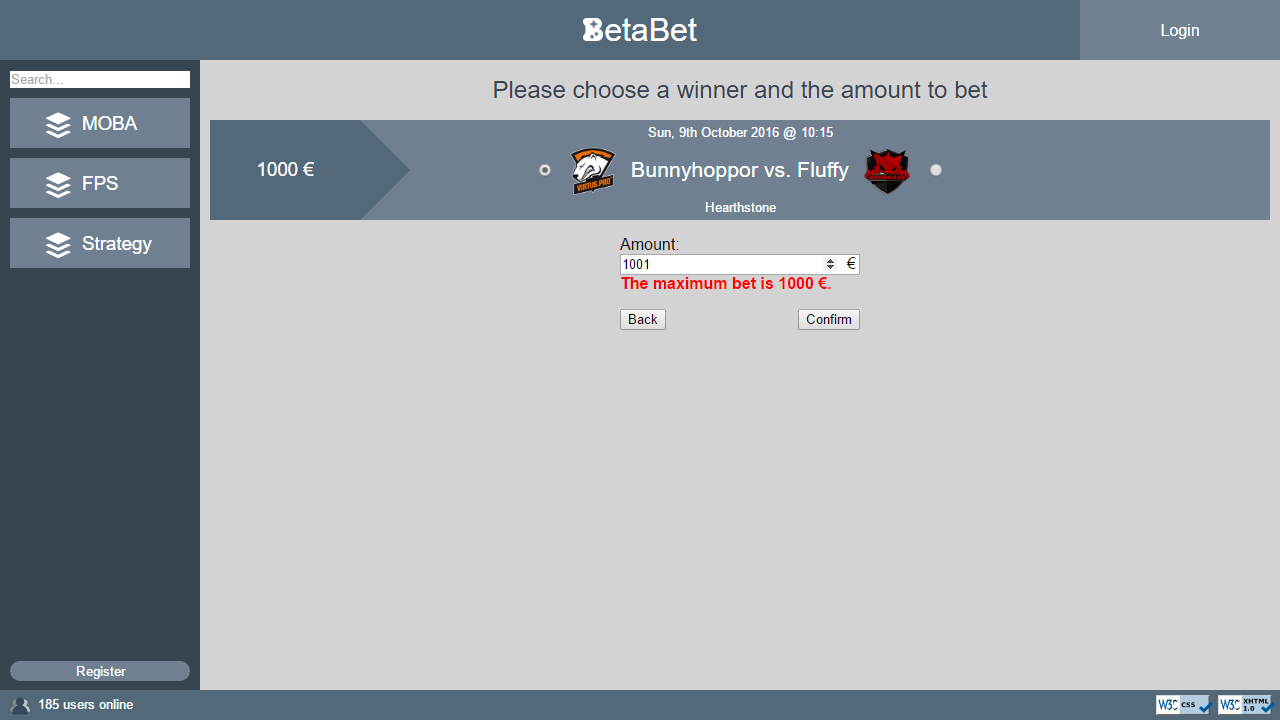
\includegraphics[width=.975\linewidth]{bet3}
        Apuesta muy grande
    \end{center}
    \columnbreak
    \begin{center}
        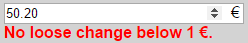
\includegraphics[width=.975\linewidth]{bet4}
        Céntimos no permitidos
    \end{center}
\end{multicols}
Cuando se confirma una apuesta válida, se muestra una confirmación y posteriormente se añade al carrito.
\smallbreak
\begin{minipage}{\linewidth}
    \centering
    \captionsetup{type=figure}
    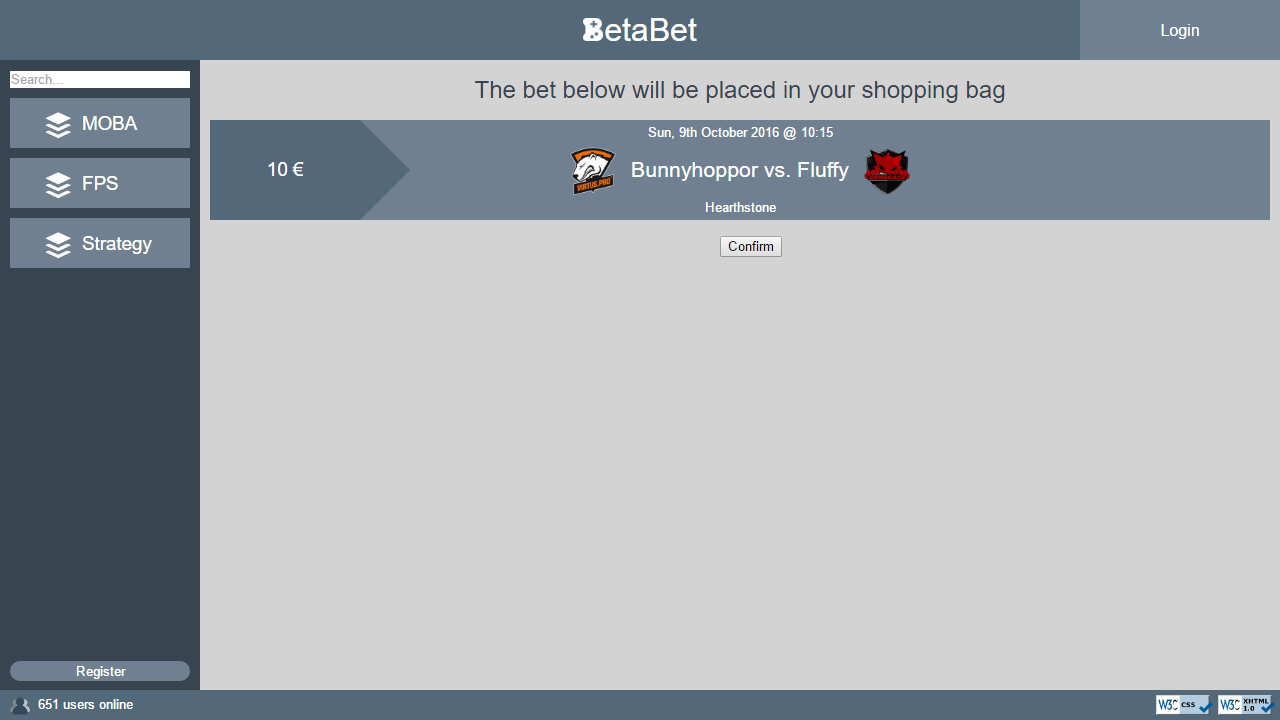
\includegraphics[width=\linewidth]{fig6}
    \caption{Confirmación de apuesta}
    \label{fig:fig6}
\end{minipage}
\smallbreak
Nota: Los botones \textit{Back} (\autoref{fig:fig5}) y \textit{Confirm} (\autoref{fig:fig6}) llevan al usuario de vuelta a la página principal.
\newpage
\subsection{Confirmar el carrito}
Si el carrito contiene una o más apuestas, aparece un botón en la esquina superior izquierda de la página indicando la cantidad total de dinero apostado. Al situar el puntero sobre este botón el texto cambia a \textit{Checkout}, y al pulsarlo se accede a la página de administración del carrito de apuestas.
\begin{center}
    \raisebox{-.5\height}{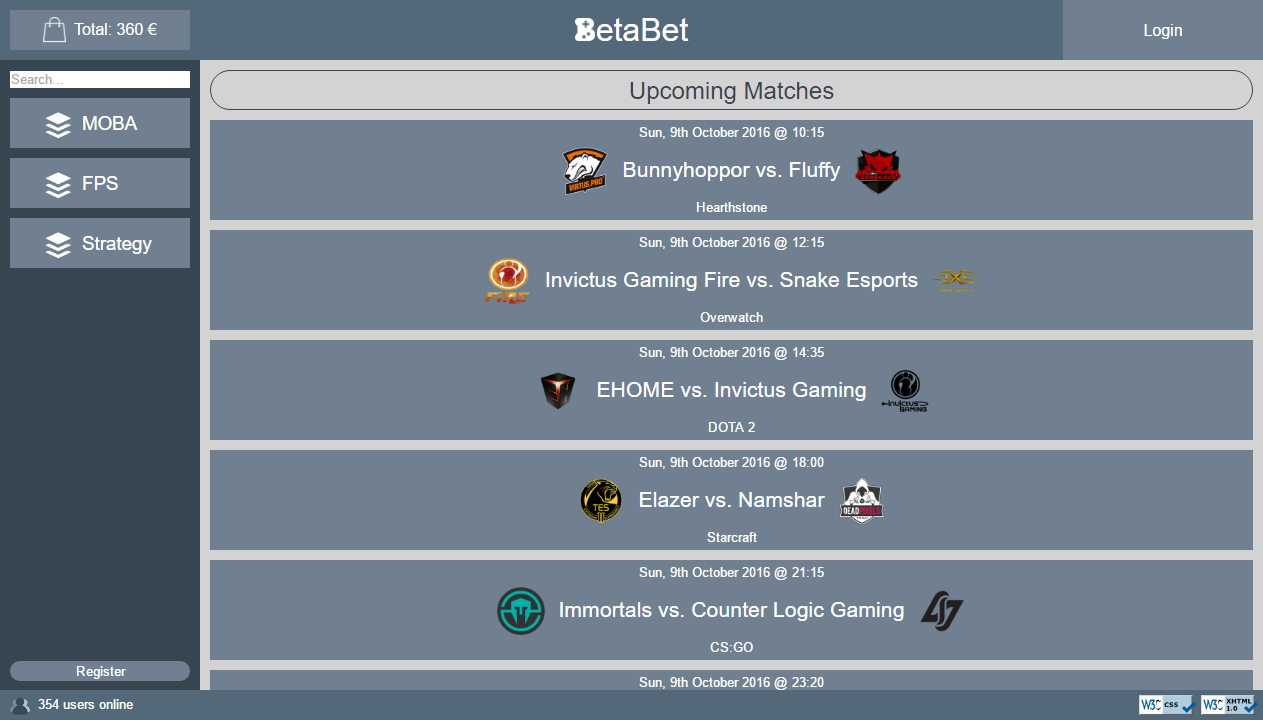
\includegraphics[width=.2\linewidth]{checkout1}}
    \raisebox{-.6\height}{\scalebox{2}{\myarrow}}
    \raisebox{-.5\height}{
\includegraphics[width=.2\linewidth]{checkout2}}
\end{center}
Esta página muestra todas las apuestas incluidas en el carrito junto con el dinero total que será apostado.
\smallbreak
\begin{minipage}{\linewidth}
    \centering
    \captionsetup{type=figure}
    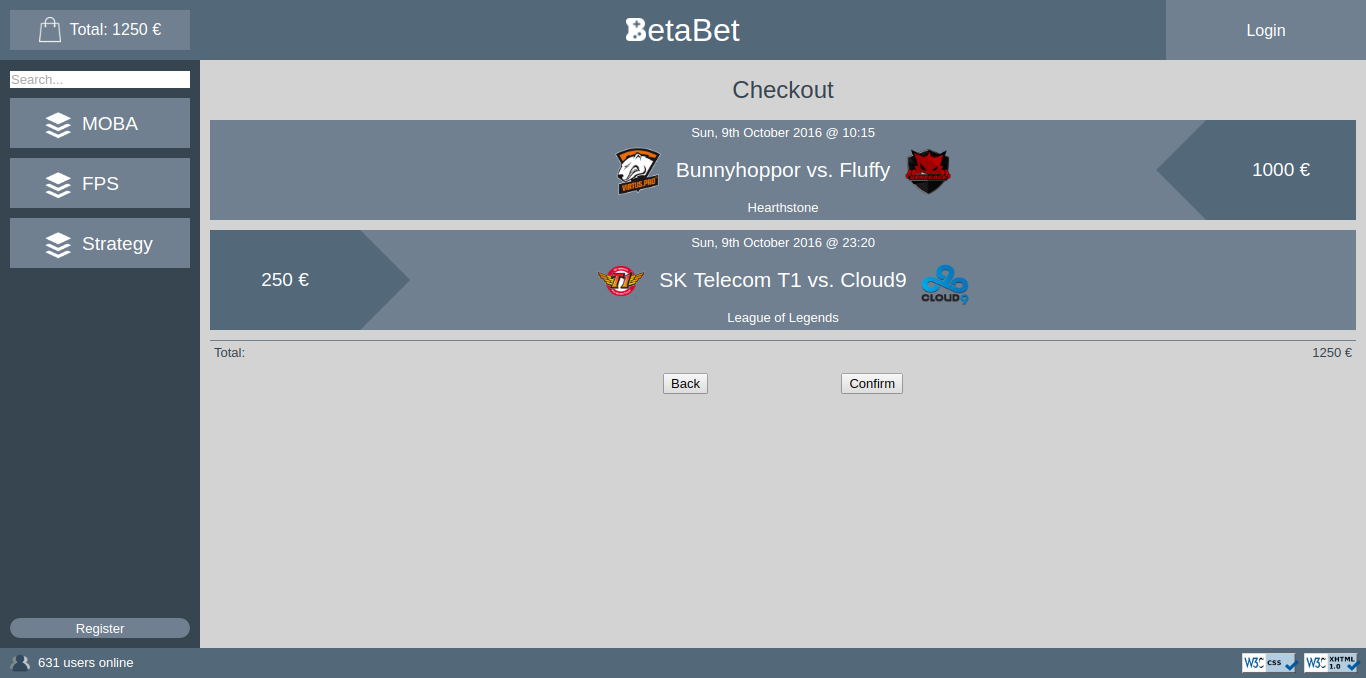
\includegraphics[width=\linewidth]{fig7}
    \caption{Carrito de apuestas}
    \label{fig:fig7}
\end{minipage}
\smallbreak
Situando el cursor sobre una apuesta del carrito, aparecen botones para modificar o eliminar dicha apuesta.
\begin{center}
    
\includegraphics[width=.8\linewidth]{checkout3}
\end{center}
La opción \textit{Edit} conduce al usuario a una página similar a \autoref{fig:fig5} que permite modificar apuesta inicial, mientras que \textit{Remove} muestra una confirmación equivalente a \autoref{fig:fig6} para eliminar la apuesta del carrito.
\smallbreak
Nota: Los botones \textit{Back} (\autoref{fig:fig5}) y \textit{Confirm} (\autoref{fig:fig6}) correspondientes en este caso vuelven a \textit{Checkout}.
\bigbreak
Cuando el usuario confirma el carrito de apuestas, se comprueba que éste haya iniciado sesión y que tenga suficiente saldo en su cuenta. En caso contrario, se muestran los avisos pertinentes en el formulario.
\begin{multicols}{3}
    \begin{center}
        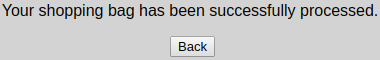
\includegraphics[width=.975\linewidth]{checkout4}
        \cmark$\;$Carrito procesado con éxito
    \end{center}
    \columnbreak
    \begin{center}
        
\includegraphics[width=.975\linewidth]{checkout5}
        \xmark$\;$No hay una sesión iniciada
    \end{center}
    \columnbreak
    \begin{center}
        
\includegraphics[width=.975\linewidth]{checkout6}
        \xmark$\;$Saldo insuficiente en la cuenta
    \end{center}
\end{multicols}
\bigbreak
Una vez el carrito ha sido procesado correctamente éste queda vacío, el saldo de la cuenta del usuario se ve decrementado convenientemente y las apuestas están disponibles en el historial de apuestas.
\newpage
\subsection{Registrar un nuevo usuario}
Si el usuario no ha iniciado sesión, aparece en la esquina inferior izquierda de la página el botón \textit{Register}, que lleva al formulario de registro de un nuevo usuario.
\smallbreak
\begin{minipage}{\linewidth}
    \centering
    \captionsetup{type=figure}
    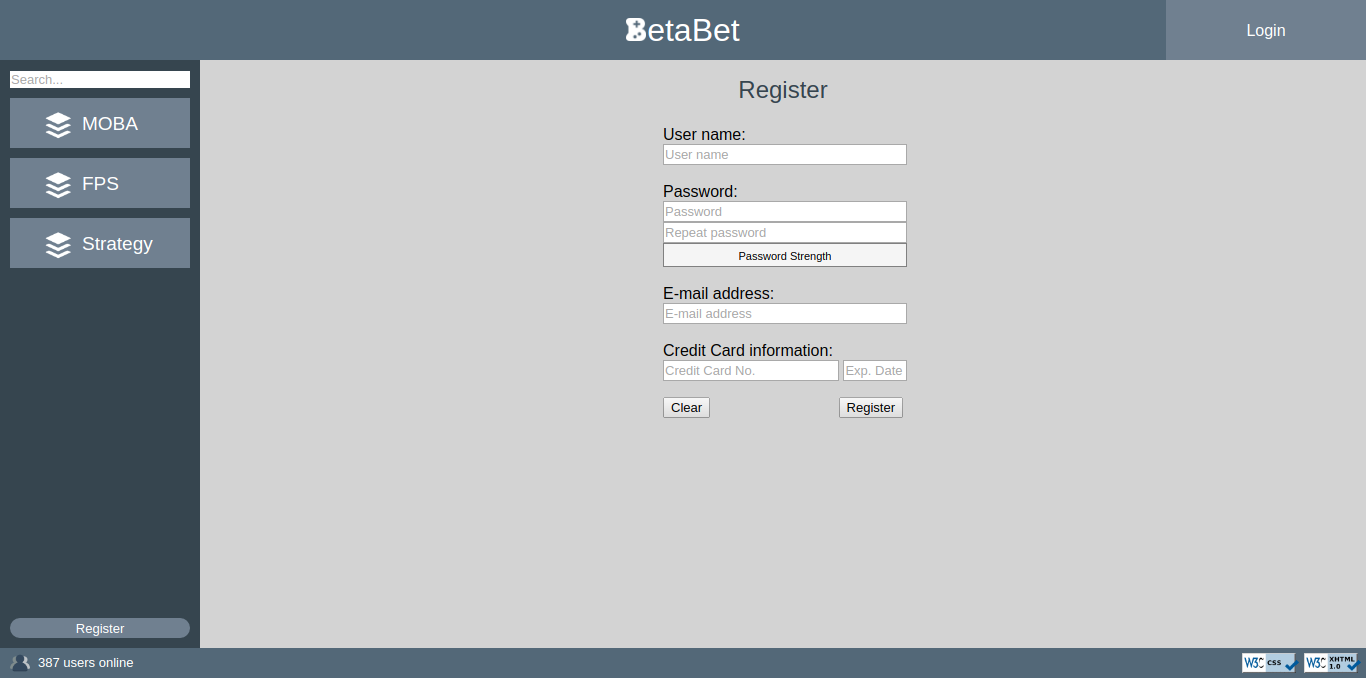
\includegraphics[width=\linewidth]{fig8}
    \caption{Formulario de registro}
    \label{fig:fig8}
\end{minipage}
\smallbreak
Al escribir en el campo \textit{Password}, el medidor de fortaleza de la contraseña se actualiza correspondientemente.
{\centering
    
\includegraphics[width=.16\linewidth]{strength1}
    
\includegraphics[width=.16\linewidth]{strength2}
    
\includegraphics[width=.16\linewidth]{strength3}
    
\includegraphics[width=.16\linewidth]{strength4}
    
\includegraphics[width=.16\linewidth]{strength5}
    
\includegraphics[width=.16\linewidth]{strength6}
}
\medbreak
El botón \textit{Register} comprueba que todos los datos introducidos son válidos. De ser así, se da la bienvenida al nuevo usuario, en otro caso se informa de los campos en los que se han introducido datos incorrectos.
\begin{multicols}{4}
    \begin{center}
        
\includegraphics[width=.975\linewidth]{register1}
        \cmark$\;$Registro con éxito
    \end{center}
    \columnbreak
    \begin{center}
        
\includegraphics[width=.975\linewidth]{register2}
        \xmark$\;$El usuario ya existe
    \end{center}
    \columnbreak
    \begin{center}
        
\includegraphics[width=.975\linewidth]{register3}
        \xmark$\;$Usuario incorrecto
    \end{center}
    \columnbreak
    \begin{center}
        
\includegraphics[width=.975\linewidth]{register4}
        \xmark$\;$Contraseña incorrecta
    \end{center}
\end{multicols}
\begin{multicols}{4}
    \begin{center}
        
\includegraphics[width=.975\linewidth]{register5}
        \xmark$\;$Contraseñas distintas
    \end{center}
    \columnbreak
    \begin{center}
        
\includegraphics[width=.975\linewidth]{register6}
        \xmark$\;$Email incorrecto
    \end{center}
    \columnbreak
    \begin{center}
        
\includegraphics[width=.975\linewidth]{register7}
        \xmark$\;$Nº Tarjeta incorrecto
    \end{center}
    \columnbreak
    \begin{center}
        
\includegraphics[width=.975\linewidth]{register8}
        \xmark$\;$Caducidad incorrecta
    \end{center}
\end{multicols}
Nota: El campo \textit{User name} del inicio de sesión (\autoref{fig:fig9}) se actualiza con aquel introducido al registrarse.
\subsection{Iniciar sesión con un usuario}
Colocando el puntero sobre el menú de \textit{Login} en la esquina superior derecha de la página, se despliega automáticamente el formulario de inicio de sesión.
\vspace{-12pt}
\begin{center}
    \begin{minipage}[t][][b]{.275\linewidth}
        
\includegraphics[width=.91\linewidth]{login1}
    \end{minipage}
    \raisebox{-2.33\height}{\scalebox{2}{\myarrow}}$\;$
    \begin{minipage}[t][][b]{.275\linewidth}
        \centering
        \captionsetup{type=figure}
        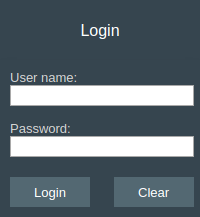
\includegraphics[width=.91\linewidth]{fig9}
        \caption{Formulario de \textit{Login}}
        \label{fig:fig9}
    \end{minipage}
\end{center}
\newpage
Si los datos introducidos son incorrectos, se informa de ello en el propio menú de \textit{Login}. En caso contrario, el menú de inicio de sesión cambia a un menú de cuenta de usuario para indicar que hay una sesión iniciada.
\vspace{-12pt}
\begin{center}
    \begin{minipage}[t][][b]{.275\linewidth}
        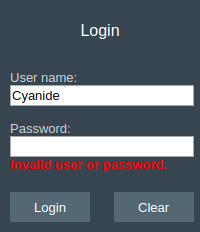
\includegraphics[width=.91\linewidth]{login2}\newline
        Datos de \textit{Login} incorrectos.
    \end{minipage}
    \hfill
    \begin{minipage}[t][][b]{.275\linewidth}
        
\includegraphics[width=.91\linewidth]{login3}
    \end{minipage}
    \raisebox{-2.33\height}{\scalebox{2}{\myarrow}}$\;$
    \begin{minipage}[t][][b]{.275\linewidth}
        \centering
        \captionsetup{type=figure}
        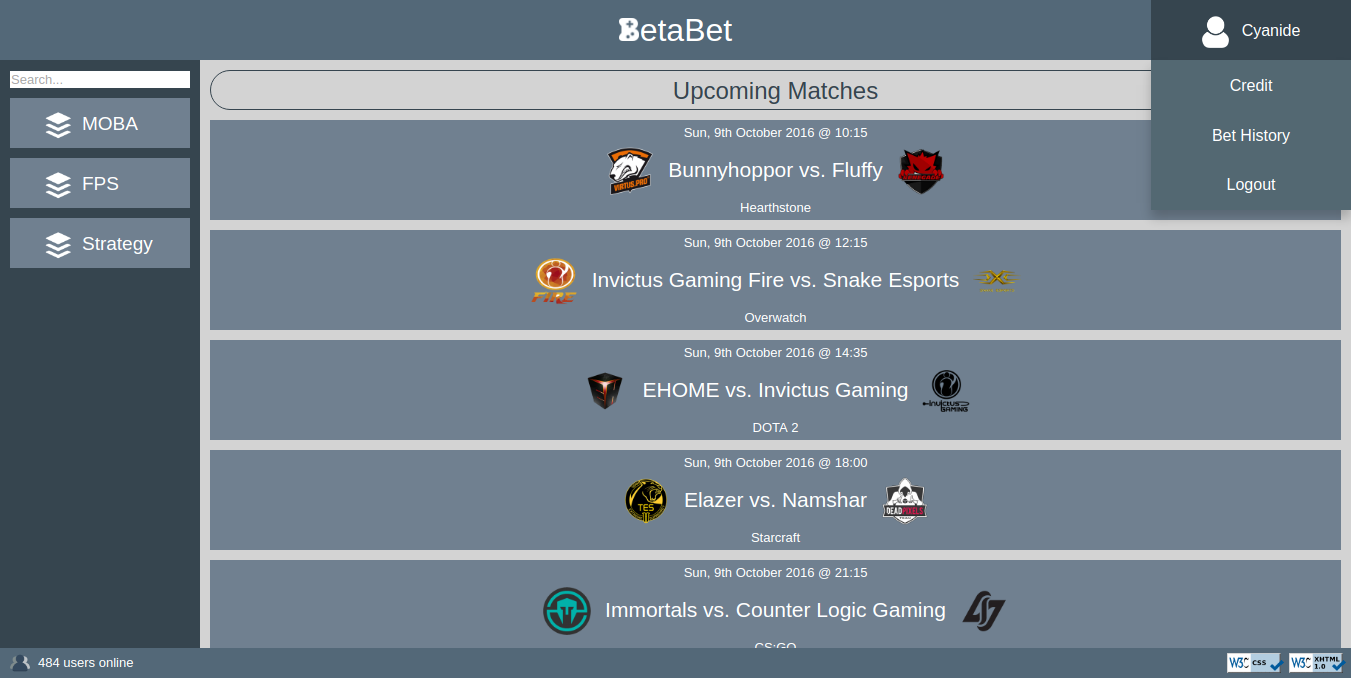
\includegraphics[width=.91\linewidth]{fig10}
        \caption{Menú del usuario}
        \label{fig:fig10}
    \end{minipage}
\end{center}
Al situar el puntero sobre este segundo menú, se despliegan las opciones principales de la cuenta (\autoref{fig:fig10}).
\smallbreak
Nota: Cada vez que un usuario inicia sesión desde su navegador, el campo \textit{User name} del inicio de sesión (\autoref{fig:fig9}) queda percargado con su nombre de usuario para la próxima vez que desee iniciar sesión.
\subsection{Consultar, ingresar y retirar saldo}
Pulsando el botón \textit{Credit} del menú de usuario (\autoref{fig:fig10}) es posible acceder a la página de administración de saldo y visualizar la cantidad actual de dinero disponible para realizar apuestas.
\smallbreak
\begin{minipage}{\linewidth}
    \centering
    \captionsetup{type=figure}
    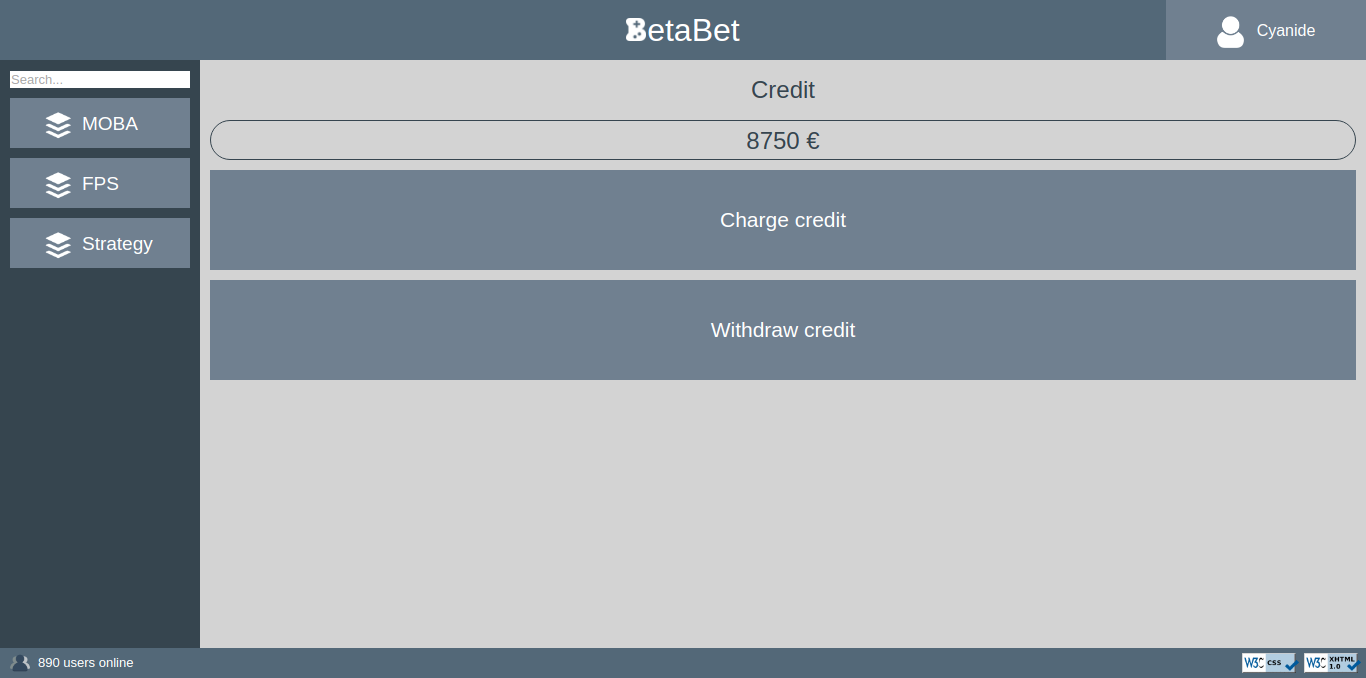
\includegraphics[width=\linewidth]{fig11}
    \caption{Administración de saldo}
    \label{fig:fig11}
\end{minipage}
\bigbreak
Para ingresar o retirar saldo basta con elegir la opción deseada (\textit{Charge} o \textit{Withdraw}, respectivamente) en esta misma página. A continuación, se solicitará al usuario la cantidad que desea ingresar o retirar de su saldo, se comprobarán los datos introducidos y finalmente se mostrará una página de confirmación mediante una interfaz muy similar a la mostrada en \autoref{fig:fig5} y \autoref{fig:fig6}.
\smallbreak
Nota: La tarjeta de crédito con la que se registra el usuario es puramente simbólica. Para fines prácticos, ingresar o retirar dinero únicamente suma o resta al saldo de la cuenta la cantidad introducida después de comprobar su formato y que no excede un umbral (o el saldo disponible, en el caso de la retirada).
\newpage
\subsection{Consultar el historial de apuestas}
De forma análoga, para consultar el historial de apuestas del usuario se utiliza el botón \textit{Bet History} del menú desplegable de usuario (\autoref{fig:fig10}). En esta página, se muestra un listado de todas las apuestas realizadas por el usuario ordenadas según el momento en el que se realizaron, empezando por las más recientes.
\smallbreak
\begin{minipage}{\linewidth}
    \centering
    \captionsetup{type=figure}
    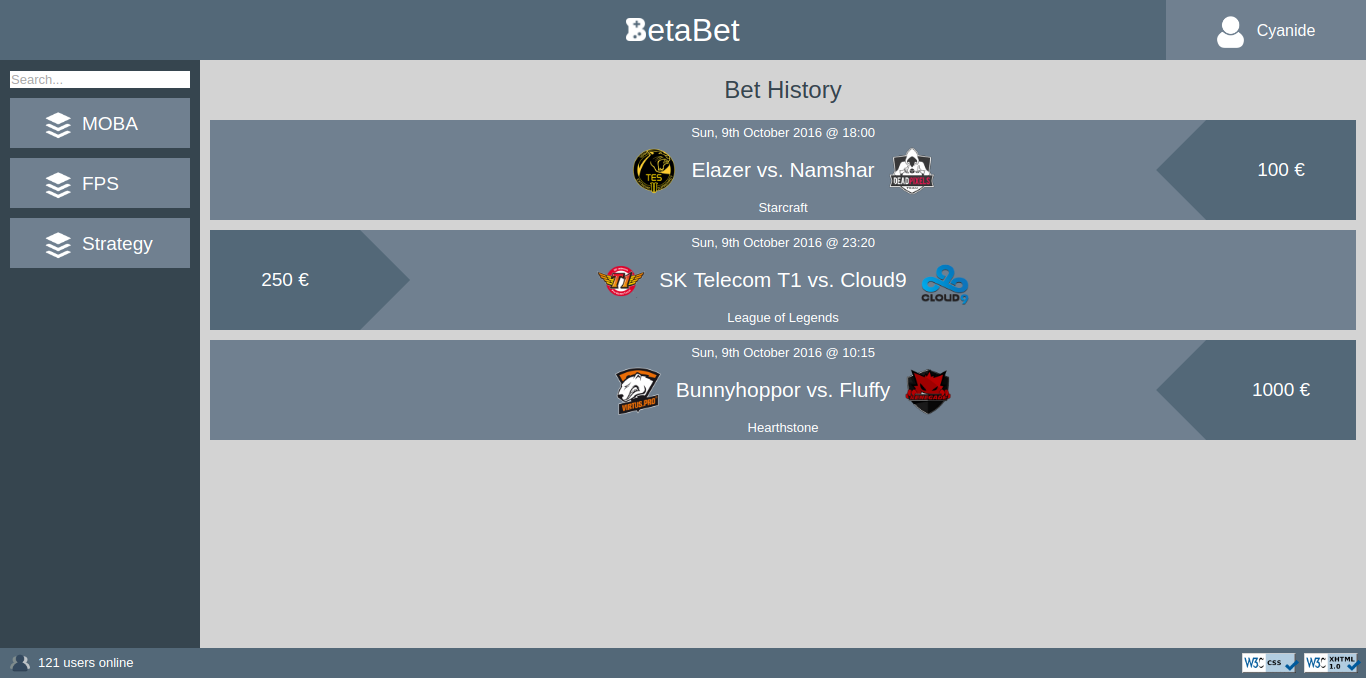
\includegraphics[width=\linewidth]{fig12}
    \caption{Historial de apuestas}
    \label{fig:fig12}
\end{minipage}
\medbreak
Pulsando cualquier apuesta del historial, se despliega información sobre el momento exacto en que se realizó.
\vspace{-16pt}
\begin{center}
    
\includegraphics[width=.8\linewidth]{history1}
\end{center}
\subsection{Cerrar la sesión}
Por último, la opción \textit{Logout} del menú de cuenta de usuario (\autoref{fig:fig10}) termina la sesión del usuario activo.
\newpage
\section{Implementación}
El sitio web está desarrollado siguiendo los siguientes criterios de implementación:
\begin{itemize}
    \item Se ha empleado un diseño modular, de manera que la vista principal \texttt{index.php} incluye la cabecera, la barra lateral y el pie de la página, mientras que en la zona de contenidos se cargan otros archivos PHP mediante peticiones AJAX según la interacción del usuario. El contador de usuarios también se actualiza automáticamente cada 3 segundos mediante AJAX.
    \item Todo el modelado visual de la página, así como algunos de los efectos utilizados, están codificados en una única hoja de estilo CSS \texttt{theme.css}, logrando así código HTML más independiente.
    \item Los datos estáticos y semi-estáticos del sitio web se almacenan en el servidor como archivos de texto \texttt{.dat} y XML, estos últimos son administrados en memoria mediante la librería SimpleXML. Todos los demás datos se manejan en forma de variables PHP, con uso exhaustivo de \textit{arrays} asociativos. El flujo de datos PHP cliente-servidor se lleva a cabo a través de métodos GET y POST de formularios, así como sesiones PHP (carrito de apuestas) y \textit{cookies} de navegación (precargado de \textit{User name}).
    \item Se utilizan funciones JavaScript en conjunto con AJAX y jQuery para gran parte de las interacciones del usuario (validación de formularios, fortaleza de la contraseña, despliegue de detalles en el historial de apuestas, etc.). El archivo \texttt{functions.js} proporciona la mayoría de estas funcionalidades.
    \item También se han configurado los campos de los formularios con los atributos HTML5 correspondientes para que el navegador notifique al usuario cuando introduce datos incorrectos.
    \item Se ha implementado un sistema de \textit{tokens} con el fin de denegar el acceso directo a los archivos PHP que se cargan dinámicamente mediante AJAX, ya que esto podría causar errores de estilo y vulnerabilidades en el sistema (por ejemplo, al escribir la ruta de \texttt{matches.php} en la barra de direcciones).
\end{itemize}
\section{Referencias}
Durante el desarrollo de esta práctica, se han seguido las siguientes referencias:
\begin{ldescription}
    \item[$\bullet$ Moodle UAM \url{https://moodle.uam.es/}]
        Enunciado y normativa de la práctica.
    \item[$\bullet$ W3Schools \url{http://www.w3schools.com/}]
        Referencias HTML, CSS, JavaScript y jQuery.
    \item[$\bullet$ PHP Manual \url{http://php.net/manual/}]
        Referencias PHP.
    \item[$\bullet$ Stack Overflow \url{http://stackoverflow.com/}]
        Consulta de dudas particulares.
    \item[$\bullet$ LaTeX \url{https://en.wikibooks.org/wiki/LaTeX}]
        Referencias LaTeX para la redacción de esta memoria.
\end{ldescription}
\end{document}
